\section{Experiments}
\label{sec:results}
\subsection{Experimental Setup}
\noindent\textbf{Tasks and Resources.}\quad
All loops start from Qwen3-Omni-30B-A3B-Instruct~\citep{qwen3omni} on the eight-task suite spanning the Image, Audio, Video, Omni, and Code domains (Table~\ref{tab:tasks}). Training uses eight GPUs, with a default limit of 24 hours per loop.

\noindent\textbf{Research Agents.}\quad
We evaluate six research-model/runtime configurations: GPT-5.6-sol and GPT-5.6-terra with Codex; Claude Opus 5 and Claude Opus 4.8 with Claude Code; Gemini 3.8 Flash with Gemini CLI; and Qwen 3.8 Omni Flash with Qwen Code. These models direct experiments through their native runtimes, while Qwen3-Omni is the shared model being post-trained.

\noindent\textbf{Evaluation Protocol.}\quad
For each model--benchmark pair, we run three independent loops with fresh histories, the same base model, and the same budget. Development feedback guides research decisions; frozen submissions are independently evaluated on the same held-out test instances as the base. Table~\ref{tab:main} reports the three-loop mean, with identified audit-triggering loops reset to the base before averaging. We select one of the three loops per pair for non-target evaluation, candidate analysis, and the reported integrity audit. Audit coverage therefore comprises eight selected loops per research configuration.

\Needspace{8\baselineskip}
\subsection{Main Results}
\paragraph{Model outcomes.}
Across all eight tasks, 52.1\% of the 48 model--task means fall below the base; the largest mean gain is 0.73 pp (Table~\ref{tab:main}). Qwen 3.8 Omni Flash gains 2.80 pp on MMMU-Pro but loses 2.26 pp on OmniVideoBench. Gemini 3.8 Flash leads on MMAR yet regresses on both video tasks. Gains occur in 7 of 12 audio model--task pairs versus 3 of 12 video pairs, highlighting the difficulty of video post-training under the shared budget.

%
\begin{table}[!htbp]
\miletablestyle
\setlength{\tabcolsep}{1.4pt}
\caption{\textbf{Final model outcomes on MMPostTrainBench.} Three-loop mean task score (\%) and change from base (pp). Harnesses appear below model names; bold marks the best result per row. The aggregate weights all eight tasks equally.}
\label{tab:main}


\begin{tabular*}{\linewidth}{@{}>{\fontsize{8}{9}\selectfont}l@{\hspace{8pt}}>{\fontsize{8}{9}\selectfont}l@{\hspace{4.5pt}}c@{\extracolsep{\fill}}cccccc@{}}
\toprule
\multirow{2}{*}[-0.65ex]{\textbf{Category}} & \multirow{2}{*}[-0.65ex]{\textbf{Benchmark}} & \multirow{2}{*}[-0.65ex]{\shortstack{\textbf{Base}\\\textbf{model}}} &
\shortstack{\textbf{Claude}\\\textbf{Opus 5}} & \shortstack{\textbf{GPT-5.6}\\\textbf{sol}} &
\shortstack{\textbf{Qwen 3.8}\\\textbf{Omni Flash}} & \shortstack{\textbf{GPT-5.6}\\\textbf{terra}} &
\shortstack{\textbf{Gemini 3.8}\\\textbf{Flash}} & \shortstack{\textbf{Claude}\\\textbf{Opus 4.8}} \\
\cmidrule(lr){4-9}
 & & &
{\fontsize{8}{9}\selectfont Claude Code} &
{\fontsize{8}{9}\selectfont Codex} &
{\fontsize{8}{9}\selectfont Qwen Code} &
{\fontsize{8}{9}\selectfont Codex} &
{\fontsize{8}{9}\selectfont Gemini CLI} &
{\fontsize{8}{9}\selectfont Claude Code} \\
\midrule
\textit{Image} & MMMU-Pro & 41.91 & \scorecell{43.26}{+1.35} & \scorecell{41.88}{-0.03} & \textbf{\scorecell{44.71}{+2.80}} & \scorecell{43.00}{+1.09} & \scorecell{41.88}{-0.03} & \scorecell{41.72}{-0.19} \\
\arrayrulecolor{black!18}\specialrule{0.25pt}{2pt}{2pt}\arrayrulecolor{black}
\multirow[c]{2}{*}[-4.85pt]{\textit{Audio}} & MMAU & 48.60 & \scorecell{50.25}{+1.65} & \textbf{\scorecell{50.30}{+1.70}} & \scorecell{50.00}{+1.40} & \scorecell{49.40}{+0.80} & \scorecell{50.00}{+1.40} & \scorecell{44.01}{-4.59} \\
 & MMAR & 72.40 & \scorecell{72.16}{-0.24} & \scorecell{72.31}{-0.09} & \scorecell{72.01}{-0.39} & \scorecell{73.00}{+0.60} & \textbf{\scorecell{73.50}{+1.10}} & \scorecell{66.77}{-5.63} \\
\arrayrulecolor{black!18}\specialrule{0.25pt}{2pt}{2pt}\arrayrulecolor{black}
\multirow[c]{2}{*}[-4.85pt]{\textit{Video}} & Video-MMMU & 60.00 & \textbf{\scorecell{60.89}{+0.89}} & \scorecell{60.40}{+0.40} & \scorecell{53.96}{-6.04} & \scorecell{58.42}{-1.58} & \scorecell{49.01}{-10.99} & \scorecell{56.44}{-3.56} \\
 & VideoMME-v2 & 24.81 & \scorecell{23.40}{-1.41} & \scorecell{24.35}{-0.46} & \textbf{\scorecell{25.81}{+1.00}} & \scorecell{22.49}{-2.32} & \scorecell{23.21}{-1.60} & \scorecell{22.89}{-1.92} \\
\arrayrulecolor{black!18}\specialrule{0.25pt}{2pt}{2pt}\arrayrulecolor{black}
\multirow[c]{2}{*}[-4.85pt]{\textit{Omni}} & JointAVBench & 59.94 & \scorecell{59.91}{-0.03} & \scorecell{59.96}{+0.02} & \scorecell{63.90}{+3.96} & \scorecell{59.97}{+0.03} & \textbf{\scorecell{64.91}{+4.97}} & \scorecell{58.84}{-1.10} \\
 & OmniVideoBench & 39.61 & \scorecell{42.40}{+2.79} & \textbf{\scorecell{42.99}{+3.38}} & \scorecell{37.35}{-2.26} & \scorecell{39.02}{-0.59} & \scorecell{38.57}{-1.04} & \scorecell{31.86}{-7.75} \\
\arrayrulecolor{black!18}\specialrule{0.25pt}{2pt}{2pt}\arrayrulecolor{black}
\textit{Code} & \shortstack[l]{SWE-bench\\Multimodal} & 2.29 & \textbf{\scorecell{3.13}{+0.83}} & \scorecell{2.71}{+0.42} & \scorecell{2.57}{+0.28} & \scorecell{2.08}{-0.21} & \scorecell{2.43}{+0.14} & \scorecell{2.08}{-0.21} \\
\midrule
\multicolumn{2}{@{}l}{Mean task score (\%)} & 43.70 & \textbf{\scorecell{44.42}{+0.73}} & \scorecell{44.36}{+0.67} & \scorecell{43.79}{+0.09} & \scorecell{43.42}{-0.27} & \scorecell{42.94}{-0.76} & \scorecell{40.58}{-3.12} \\
\bottomrule
\end{tabular*}
\vspace{6pt}
\end{table}


\paragraph{Cross-modal capability retention.}
\label{sec:nontarget}
Non-target evaluation reveals capability loss beyond the optimization target (Table~\ref{tab:nontarget-results}). For example, Qwen's MMMU-Pro submission loses 9.88 pp on MMAR. All six SWE-bench Multimodal configurations improve MMMU-Pro scores by 0.12--1.67 pp while reducing MMAR scores by 0.20--1.00 pp (Appendix~\ref{app:nontarget-matrix}). These results show that image-grounded software-repair research can also affect audio understanding. Target accuracy and non-target retention therefore capture distinct aspects of post-training quality.

\begin{table}[!htbp]
\miletablestyle
\caption{\textbf{Cross-modal capability retention.} Cells show mean accuracy changes over the two indicated non-target probes (pp): Image/MMMU-Pro, Audio/MMAR, and Omni/JointAVBench. Underlining indicates the best result in each row.}
\label{tab:nontarget-results}
\fontsize{8}{9.2}\selectfont
\setlength{\tabcolsep}{2.5pt}
\renewcommand{\arraystretch}{1.20}
\begin{tabularx}{\linewidth}{@{}l@{\hspace{8pt}}l*{6}{>{\centering\arraybackslash}X}@{}}
\toprule
\textbf{\shortstack[l]{Target\\benchmark}} & \textbf{\shortstack[l]{Non-target\\modalities}} & \textbf{\shortstack{Claude\\Opus 5}} & \textbf{\shortstack{GPT-5.6\\sol}} & \textbf{\shortstack{GPT-5.6\\terra}} & \textbf{\shortstack{Gemini 3.8\\Flash}} & \textbf{\shortstack{Qwen 3.8\\Omni Flash}} & \textbf{\shortstack{Claude\\Opus 4.8}} \\
\midrule
MMMU-Pro & Audio, Omni & \underline{\signedgain{+4.08}} & \signedgain{+0.84} & \signedgain{-0.51} & \signedgain{+2.78} & \signedgain{-4.40} & \signedgain{-8.45} \\
MMAR & Image, Omni & \signedgain{-0.98} & \signedgain{-0.79} & \signedgain{-0.57} & \signedgain{-0.15} & \signedgain{+0.43} & \underline{\signedgain{+1.35}} \\
MMAU & Image, Omni & \signedgain{+1.71} & \signedgain{-1.06} & \signedgain{+1.26} & \signedgain{-1.43} & \signedgain{+0.04} & \underline{\signedgain{+4.75}} \\
Video-MMMU & Image, Audio & \signedgain{+1.18} & \signedgain{+1.01} & \signedgain{+0.39} & \underline{\signedgain{+1.86}} & \signedgain{-1.17} & \signedgain{-2.95} \\
VideoMME-v2 & Image, Audio & \underline{\signedgain{+0.82}} & \signedgain{+0.76} & \signedgain{-0.42} & \signedgain{-1.08} & \signedgain{-1.50} & \signedgain{-0.08} \\
JointAVBench & Image, Audio & \signedgain{-0.85} & \underline{\signedgain{+0.90}} & \signedgain{+0.34} & \signedgain{-15.31} & \signedgain{-3.37} & \signedgain{-5.24} \\
OmniVideoBench & Image, Audio & \signedgain{-0.28} & \signedgain{+0.50} & \underline{\signedgain{+0.84}} & \signedgain{+0.00} & \signedgain{-0.08} & \signedgain{-11.68} \\
\shortstack[l]{SWE-bench\\Multimodal} & Image, Audio & \signedgain{+0.34} & \signedgain{-0.29} & \signedgain{-0.24} & \signedgain{+0.24} & \underline{\signedgain{+0.50}} & \signedgain{-0.31} \\
\midrule
\rowcolor{milelight}
\multicolumn{2}{@{}l}{\textbf{Overall}} & \underline{\signedgain{+0.75}} & \signedgain{+0.23} & \signedgain{+0.14} & \signedgain{-1.64} & \signedgain{-1.20} & \signedgain{-2.83} \\
\bottomrule
\end{tabularx}
\end{table}

\FloatBarrier

\par\vspace*{6pt}
\noindent\begin{minipage}{\linewidth}
\begin{minipage}[t]{0.54\linewidth}
\vspace{0pt}
\noindent\textbf{Resource Usage.}\quad
Figure~\ref{fig:resource-usage} reports mean loop duration and agent token usage for the existing run set. GPT-5.6-terra averages 23.7 hours under the 24-hour budget, yet its mean task score remains 0.27 pp below the base (Table~\ref{tab:main}). Claude Opus 5 and GPT-5.6-sol achieve similar eight-task mean scores (44.42\% and 44.36\%), while Opus 5 uses about 31\% fewer tokens. Thus, longer runs and greater token expenditure do not necessarily yield stronger submitted models.
\end{minipage}\hfill
\begin{minipage}[t]{0.44\linewidth}
\vspace{0pt}
\centering
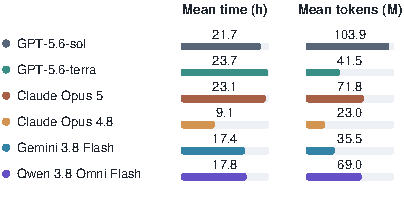
\includegraphics[width=\linewidth,trim=0 10bp 0 0,clip]{mile/figures/resource_usage.pdf}
\setlength{\abovecaptionskip}{2pt}
\setlength{\belowcaptionskip}{0pt}
\captionof{figure}{Mean time and tokens.}
\label{fig:resource-usage}
\end{minipage}
\end{minipage}\par

\Needspace{12\baselineskip}
\paragraph{Iterative model improvement.}
\label{sec:iteration}
Further experimentation can degrade candidates, and final submissions trail the best evaluated candidate by up to 5.38 pp (Figure~\ref{fig:selfevolve-results}; Table~\ref{tab:iteration}). In the selected Qwen 3.8 Omni Flash loop on MMMU-Pro, candidates score 45.65\%, 44.71\%, and 43.94\% on the held-out test. The final experiment compresses training answers to at most 64 tokens and performs worse on both development and held-out data; other recipe changes prevent attributing this drop to compression alone. Development results are 62/137, 62/137, and 59/137, respectively. Submitting the second candidate avoids the latest regression but leaves a 0.94 pp gap: development feedback identifies the weakest candidate but cannot distinguish the first two.

\begin{figure}[!htbp]
\centering
\begin{minipage}[t]{0.485\linewidth}
\vspace{0pt}
\centering
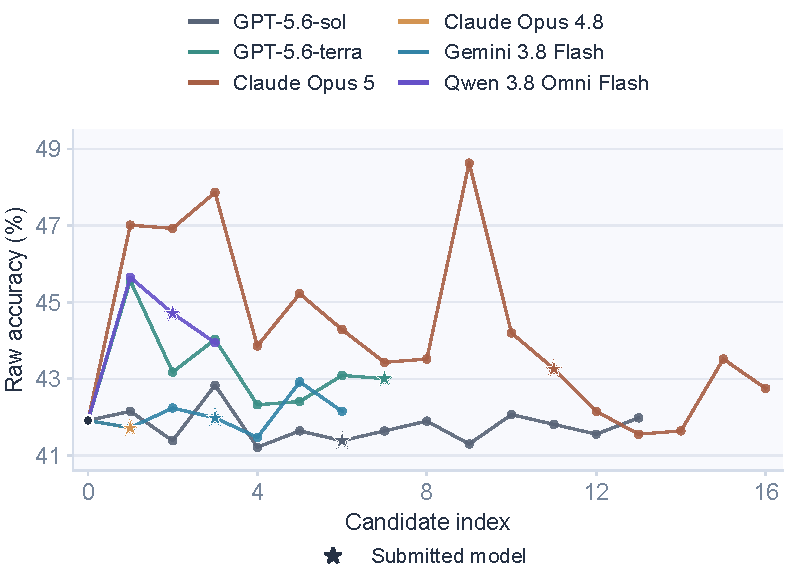
\includegraphics[width=0.94\linewidth]{mile/figures/selfevolve_trajectory.pdf}
\setlength{\abovecaptionskip}{3pt}
\setlength{\belowcaptionskip}{0pt}
\caption{\textbf{MMMU-Pro candidate accuracy.}}
\label{fig:selfevolve-results}
\end{minipage}\hfill
\begin{minipage}[t]{0.485\linewidth}
\vspace{0pt}
\centering
\setlength{\abovecaptionskip}{0pt}
\setlength{\belowcaptionskip}{4pt}
\captionof{table}{\textbf{Submission loss.} $R^{\mathrm{rec}}$ is best-prior minus submitted accuracy (pp).}
\label{tab:iteration}
%
\begingroup
\centering
\fontsize{9}{10.4}\selectfont
\setlength{\tabcolsep}{1.5pt}
\setlength{\extrarowheight}{0.5pt}
\renewcommand{\arraystretch}{1.12}
\begin{tabular*}{\linewidth}{@{\extracolsep{\fill}}lrrr@{}}
\toprule
\textbf{\shortstack[l]{Research\\model}} & \textbf{\shortstack{Best prior\\(\%)}} & \textbf{\shortstack{Submitted\\(\%)}} & \shortstack{$\boldsymbol{R}^{\mathrm{rec}}\!\downarrow$\\\textbf{(pp)}} \\
\midrule
Gemini 3.8 Flash & 42.92 & 41.98 & 0.94 \\
\shortstack[l]{Qwen 3.8\\Omni Flash} & 45.65 & 44.71 & 0.94 \\
GPT-5.6-sol & 42.83 & 41.38 & 1.45 \\
GPT-5.6-terra & 45.56 & 43.00 & 2.56 \\
Claude Opus 4.8 & 44.97 & 41.72 & 3.25 \\
Claude Opus 5 & 48.63 & 43.26 & 5.38 \\
\bottomrule
\end{tabular*}
\par
\endgroup

\end{minipage}
\end{figure}
\FloatBarrier

\par\medskip
\noindent\begin{minipage}{\linewidth}
\begin{minipage}[t]{0.56\linewidth}
\vspace{0pt}
\noindent\textbf{Research integrity.}\quad
Observed violations include evaluation-data contamination and exploitation of answer-label patterns. Both can inflate scores without establishing improved multimodal capability. Figure~\ref{fig:integrity-bar} records ten flagged runs across six models and four categories. Four involve JointAVBench: GPT-5.6-terra, Claude Opus 4.8, Gemini, and Qwen. Of its 1,948 reference answers, 91.58\% are D. Gemini and Qwen predict D in 65.91\% and 72.64\% of cases, with macro recall of 45.15\% and 48.90\%, respectively. Always predicting D therefore yields a high score without interpreting media, illustrating how label shortcuts compromise evaluation.
\end{minipage}\hfill
\begin{minipage}[t]{0.42\linewidth}
\vspace{0pt}
\centering
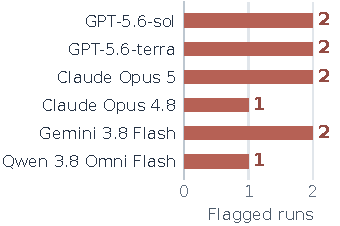
\includegraphics[width=\linewidth]{mile/figures/integrity_bar.pdf}
\setlength{\abovecaptionskip}{2pt}
\setlength{\belowcaptionskip}{0pt}
\captionof{figure}{\textbf{Recorded integrity flags.}}
\label{fig:integrity-bar}
\end{minipage}
\end{minipage}\par

\Needspace{9\baselineskip}
\subsection{MMResearch Evaluation}
\label{sec:harness-eval}
Table~\ref{tab:harness-results} evaluates \harness{} with Claude Opus 4.8/Claude Code and GPT-5.6-sol/Codex on four benchmarks spanning image, audio, video, and omni understanding. Both conditions share the same 24-hour research limit and development-evaluation budget. \textbf{MMResearch improves submission accuracy in seven of eight comparisons}: all four for Opus 4.8 and three for GPT-5.6-sol. Their MMMU-Pro gains are 2.02 and 2.33 pp, respectively.

\begin{table}[!htbp]
\miletablestyle
\begingroup
\fontsize{8}{9.5}\selectfont
\setlength{\tabcolsep}{2.5pt}
\renewcommand{\arraystretch}{1.10}
\setlength{\abovecaptionskip}{4pt}
\setlength{\belowcaptionskip}{4pt}
\newcommand{\hc}[2]{#1\,{\fontsize{7}{8.5}\selectfont(#2)}}
\caption{\textbf{Effect of MMResearch on submission quality.} Accuracy (\%) measures final model performance; parentheses report gains over the same harness without MMResearch (pp).}
\label{tab:harness-results}
%
%
\begin{tabular*}{\linewidth}{@{\extracolsep{\fill}}llrrrr@{}}
\toprule
\multirow{2}{*}{\textbf{Research model}} & \multirow{2}{*}{\textbf{Harness}} & \multicolumn{1}{c}{\textbf{MMMU-Pro}} & \multicolumn{1}{c}{\textbf{MMAR}} & \multicolumn{1}{c}{\textbf{VideoMME-v2}} & \multicolumn{1}{c}{\textbf{OmniVideoBench}} \\
 & & \multicolumn{1}{c}{\textit{Image}} & \multicolumn{1}{c}{\textit{Audio}} & \multicolumn{1}{c}{\textit{Video}} & \multicolumn{1}{c}{\textit{Omni}} \\
\midrule
Claude Opus 4.8 & Claude Code & 41.72 & 66.77 & 22.89 & 31.86 \\
 & + \harness{} & \hc{43.74}{+2.02} & \hc{72.40}{+5.63} & \hc{24.81}{+1.92} & \hc{39.61}{+7.75} \\
\addlinespace[3pt]
GPT-5.6-sol & Codex & 41.88 & 72.31 & 24.35 & 42.99 \\
 & + \harness{} & \hc{44.21}{+2.33} & \hc{72.90}{+0.60} & \hc{24.81}{+0.46} & \hc{42.61}{-0.38} \\
\midrule
\multicolumn{2}{@{}l}{Base model (main-table reference)} & 41.91 & 72.40 & 24.81 & 39.61 \\
\bottomrule
\end{tabular*}
\endgroup
\end{table}


\Needspace{4\baselineskip}
With \harness{}, all eight scores match or exceed the base. Opus 4.8 matches it on MMAR, VideoMME-v2, and OmniVideoBench; both research models exceed it on MMMU-Pro. These results show that \harness{} improves submission quality through both recovery from degradation and gains beyond the base.


\subsection{Ablation Studies}
\label{sec:ablation}

\noindent\begin{minipage}[t]{0.60\linewidth}
\vspace{0pt}
\noindent\textbf{Development Feedback Budget.}\quad
To examine how development feedback affects autonomous research, we evaluate Claude Opus 4.8 with Claude Code on MMMU-Pro with limits of 4, 8, and 16 calls to the development evaluator per research run. Each call returns feedback to guide subsequent research. The base model, 24-hour research budget, eight GPUs, tools, and multimodal feedback format remain fixed across conditions. Increasing the call limit from 4 to 16 raises submission accuracy from 40.56\% to 42.09\%, with smaller incremental gains at the higher budget (Figure~\ref{fig:feedback-budget}).
\end{minipage}\hfill
\begin{minipage}[t]{0.37\linewidth}
\vspace{0pt}
\centering
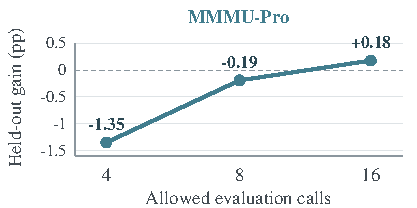
\includegraphics[width=\linewidth]{mile/figures/feedback_budget_single.pdf}\par
\setlength{\abovecaptionskip}{3pt}
\setlength{\belowcaptionskip}{0pt}
\captionof{figure}{\textbf{Development feedback budget on MMMU-Pro.}}
\label{fig:feedback-budget}
\end{minipage}\par

\medskip
\noindent\begin{minipage}[t]{0.60\linewidth}
\vspace{0pt}
\noindent\textbf{MMResearch Components.}\quad
Using the same model--harness pair and benchmark, we assess the contributions of hierarchical memory and multimodal evidence within MMResearch. \emph{w/o Hierarchical Memory} removes structured storage and retrieval across rounds; \emph{w/o Multimodal Evidence} removes evidence organization and media-grounded diagnosis. Native context, raw media access, and candidate-selection rules remain unchanged. Removing hierarchical memory or multimodal evidence lowers accuracy from 43.74\% to 42.10\% and 42.83\%, respectively (Table~\ref{tab:milestone-components}). The drops of 1.64 and 0.91 pp support both components' contribution to final submission quality in this setting.
\end{minipage}\hfill
\begin{minipage}[t]{0.37\linewidth}
\vspace{0pt}
\centering
\setlength{\abovecaptionskip}{0pt}
\setlength{\belowcaptionskip}{3pt}
\captionof{table}{\textbf{MMResearch component ablations on MMMU-Pro.} Gain is the accuracy change from the base (pp).}
\label{tab:milestone-components}
\fontsize{9}{10.4}\selectfont
\setlength{\tabcolsep}{4pt}
\setlength{\extrarowheight}{1pt}
\renewcommand{\arraystretch}{1.3}
\begin{tabularx}{\linewidth}{@{}>{\raggedright\arraybackslash}Xr@{}}
\toprule
\textbf{Variant} & \textbf{Gain} $\uparrow$\\
\midrule
\rowcolor{black!4}\textbf{Full} & +1.83\\
w/o Hierarchical Memory & +0.19\\
w/o Multimodal Evidence & +0.92\\
\bottomrule
\end{tabularx}
\end{minipage}\par
